\documentclass{beamer}
\usetheme[logo=figures/brasaoUFSC.png]{fibeamer}
%% These macros specify information about the presentation
\title{De Fortran a Julia: Computação Científica no Mundo Real}
\subtitle{QConSP 2019}
\author{Melissa Weber Mendonça}
%% These additional packages are used within the document:
\usepackage{ragged2e}  % `\justifying` text
\usepackage{booktabs}  % Tables
\usepackage{tabularx}
\usepackage{tikz}      % Diagrams
\usetikzlibrary{calc, shapes, backgrounds, }
\usepackage{pgfplots}
\usepackage{amsmath, amssymb}
\usepackage{url}       % `\url`s
\usepackage{listings}  % Code listings
\usepackage{verbatim}
\usepackage{animate}
\usepackage{hyperref}
\hypersetup{
    colorlinks = true,
    allcolors = [rgb]{1,0.83,0.39}
}
\frenchspacing

\makeatletter
\setlength\fibeamer@lengths@logowidth{4em}
\setlength\fibeamer@lengths@logoheight{5em}
\makeatother

%% Abstract:
% Hoje em dia, quando se fala Computação Científica é comum que se pense em Data Science. No entanto, existe muito mais no mundo da computação científica que não se conhece fora do nicho da matemática aplicada. Nesta palestra, falaremos sobre os fundamentos da computação científica, sua história e a importância das implementações clássicas dos algoritmos básicos de Álgebra Linear Numérica para o desenvolvimento de diversas áreas da computação. Exploraremos também algumas aplicações destas técnicas, incluindo High Performance Computing (Computação de Alto Desempenho) e algumas técnicas usadas por cientistas e Engenheiros de Software Científico (Research Software Engineers) no desenvolvimento de aplicações científicas. Finalmente, discutiremos o surgimento de linguagens mais modernas, em especial Python e Julia, suas vantagens e desvantagens para a computação científica.
%%

\begin{document}
\frame{\maketitle}

\begin{darkframes}
  \section{Scientific Computing}
  
  \begin{frame}{Quem sou eu?}
    \begin{center}
      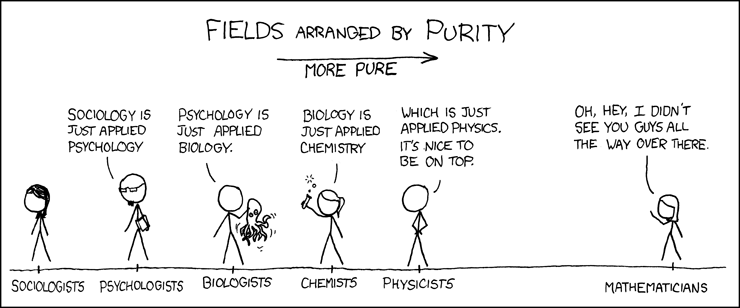
\includegraphics[width=10cm]{figures/purity.png}
    \end{center}
  \end{frame}
  
  \begin{frame}[fragile]{O que é Computação Científica?}
    \begin{center}
      \alert{Computação Científica não é só Data Science!!!!1!1ONE}
    \end{center}
    \vfill
    \begin{center}
      \verb+\includegraphics{angry.gif}+
    \end{center}
  \end{frame}
  
  \begin{frame}{O que é Computação Científica?}
    \begin{block}{}
      ``Computação Científica é a coleção de ferramentas, técnicas e teorias necessárias para a resolução computacional de modelos matemáticos de problemas nas Ciências e na Engenharia.'' \cite{GolubOrtega}
    \end{block}
    \begin{itemize}
    \item<2-> Previsão/modelagem de sistemas complexos em grande escala;
    \item<3-> Simulação de experimentos caros/perigosos;
    \item<4-> Soluções interdisciplinares de problemas das Ciências e da Engenharia.
    \item<5> ``A Computação Científica é hoje o “terceiro pilar da ciência”, ao lado da análise teórica e dos experimentos para a descoberta científica.'' \cite{TUKweb}
    \end{itemize}
  \end{frame}

  %%%%%%%%%%%%%
  % Nice quote:
  % "A majority of these tools, techniques, and theories originally developed in Mathematics, many of them having their genesis long before the advent of electronic computers. This set of mathematical theories and techniques is called Numerical Analysis (or Numerical Mathematics) and constitutes a major part of scientific computing. The development of the electronic computer, however, signaled a new era in the approach to the solution of scientific problems. Many of the numerical methods that had been developed for the purpose of hand calculation (including the use of desk calculators for the actual arithmetic) had to be revised and sometimes abandoned. Considerations that where irrelevant or unimportant for hand calculation now became of utmost importance for the efficient and correct use of a large Computer System. Many of these considerations – programming languages, operating systems, management of large quantities of data, correctness of programs – were subsumed under the new discipline of Computer Science, on which scientific computing now depends heavily. But mathematics itself continues to play a major role in scientific computing: it provides the language of the mathematical models that are to be solved and information about the suitability of a model (Does it have a solution? Is the solution unique?) and it provides the theoretical foundation for the numerical methos and, increasingly, many of the tools from computer science.
  % In summary, then, scientific computing draws on mathematics and computer science to develop the best way to use computer systems to solve problems from science and engineering."
  % -- Gene H. Golub and James M. Ortega. Scientific Computing and Differential Equations – An Introduction to Numerical Methods. Academic Press, 1992.
  %%%%%%%%%%%%% 
  
  \begin{frame}[fragile]{O que é Computação Científica?}
    \begin{center}
      \begin{tikzpicture}
        \begin{scope}[blend group = multiply]
          \fill[red!40!white]   ( 90:1) circle (1.4);
          \fill[green!40!white] (210:1) circle (1.4);
          \fill[blue!40!white]  (330:1) circle (1.4);
        \end{scope}
        \node at (0, 2.7)    {Ciência da Computação};
        \node at (-3.1, -1.5) {Matemática};
        \node at (-3.1, -2) {(algoritmos/modelagem)};
        \node at (3.8, -1.5)   {Ciências/Engenharia};
        \node at (4,2) [font=\Large] {\underline{Computação Científica}};
        \path[draw, very thick] (0,0) -- (4,1.7); 
      \end{tikzpicture}
    \end{center}
  \end{frame}
  
  \begin{frame}{Mas, na prática...}
    \begin{center}
      \begin{tikzpicture}
        \draw[very thick, white] (0,0) -- (4,0) -- (2, 3.5) -- (0,0);
        \draw[thick, white] (2,0) -- (2,1.3);
        \draw[thick, white] (2,1.3) -- (1,1.8);
        \draw[thick, white] (2,1.3) -- (3,1.8);
        \node at (2,4) {Computação Científica};
        \node at (-0.5, -0.5) {Ciência da Computação};
        \node at (4.5, -0.5) {Engenharia de Software};
        \only<2->{\path[draw=white, very thick, fill=green!30!white] (0,0) -- (2,0) -- (2,1.3) -- (1,1.75) -- (0,0);}
        \only<2->{\node[font=\scriptsize] at (-0.9, 0.9) {código rápido e bonito};}
        \only<3->{\path[draw=white, very thick, fill=blue!30!white] (2,0) -- (4,0) -- (3,1.75) -- (2,1.3) -- (2,0);}
        \only<3->{\node[font=\scriptsize] at (4.7, 0.9) {código rápido e feio};}
        \only<4->{\path[draw=white, very thick, fill=red!30!white] (2,3.5) -- (3,1.75) -- (2,1.3) -- (1,1.75) -- (2,3.5);}
        \only<4->{\node[font=\scriptsize] at (3.6, 3) {código lento e feio :(};}
      \end{tikzpicture}
    \end{center}
    
    \vfill
    \hrule
    \vskip0.15cm
    \scriptsize{Baseado na imagem \hyperlink{https://agilescientific.com/blog/2018/1/10/what-is-scientific-computing}{daqui}}
  \end{frame}
  
  \section{Aplicações}
  
  \begin{frame}{Tipos de Problemas}
    \begin{itemize}
    \item Solução Numérica de equações diferenciais: finanças, bioinformática, meteorologia, economia, física
    \item Estimação de parâmetros/Problemas inversos: estatística, Data Science, processamento de imagens, biomedicina, ajuste de curvas
    \item Simulações: física, engenharia, geociências, ciência de materiais, dinâmica de fluidos
    \item Otimização e Álgebra Linear Numérica
    \end{itemize}
  \end{frame}
  
  \begin{frame}
    \frametitle{A importância da Álgebra Linear}
    \begin{block}{Dimensão}
      Número de variáveis de um problema.
    \end{block}
    \vfill
    Exemplo:
    \begin{equation*}
      \left\{ \begin{aligned}
          2x+3y &= 1\\
          x-2y &= 1
        \end{aligned}\right.
      \only<2->{\Leftrightarrow
        \begin{pmatrix}
          2 & 3\\
          1 & -2
        \end{pmatrix}
        \begin{pmatrix} x\\y\end{pmatrix}
        = \begin{pmatrix}1\\1\end{pmatrix}}
      \only<3>{\Leftrightarrow Ax=b.}
    \end{equation*}
  \end{frame}
  
  \begin{frame}
    \frametitle{A importância da Álgebra Linear}
    A Álgebra Linear estuda espaços vetoriais e matrizes para resolver problemas do tipo
    $$Ax=b$$
    $$(A\in {\mathbb{R}}^{m\times n}, x\in {\mathbb{R}}^n, b \in {\mathbb{R}}^m)$$
    \vfill
    \only<2->{%
      \begin{center}
        \begin{minipage}{6cm}
          \begin{block}{FUN FACT:}
            \begin{center}
              A solução de todos os problemas mencionados previamente dependem da solução de sistemas lineares!
            \end{center}
          \end{block}
        \end{minipage}
      \end{center}
    }
  \end{frame}
  
  \section{Álgebra Linear Numérica}
  
  \begin{frame}{O que é Álgebra Linear Numérica?}
    \begin{center}
      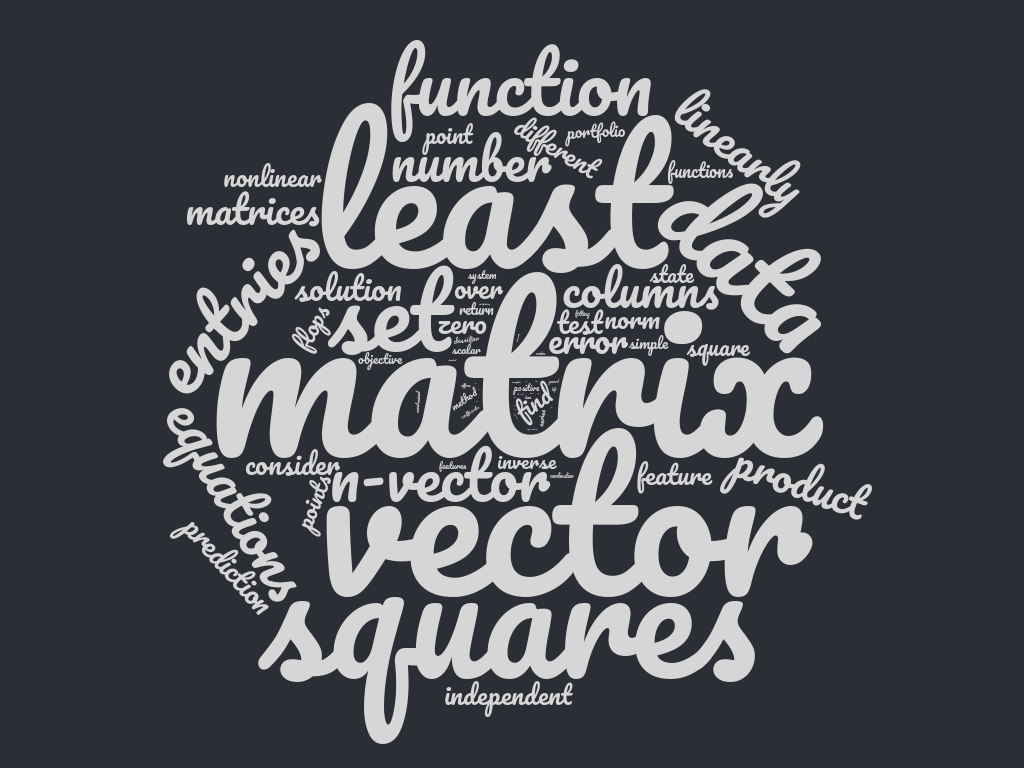
\includegraphics[width=10cm]{figures/wordcloud.png}
    \end{center}
  \end{frame}
  
  \begin{frame}{Álgebra Linear Numérica}
    Estudo de algoritmos para realizar cálculos computacionais de álgebra linear, principalmente operações em matrizes e vetores.
    \vfill
    Algoritmos principais:
    \begin{itemize}
    \item Decomposição LU
    \item Decomposição QR
    \item Decomposição em Valores Singulares (SVD - usado em PCA)
    \item Cálculo de Autovalores/Autovetores
    \item Métodos iterativos especializados para a resolução de sistemas lineares
    \end{itemize}
  \end{frame}
  
  \section{Ferramentas}
  
  \begin{frame}
    \frametitle{BLAS (1979)}
    \emph{Basic Linear Algebra Subprograms} (BLAS): especificação de rotinas de baixo nível para operações comuns de álgebra linear. %\hyperref[\url{https://en.wikipedia.org/wiki/Basic_Linear_Algebra_Subprograms}]{(Wikipedia)}
    \begin{itemize}
    \item ATLAS
    \item MKL
    \item OpenBLAS (GotoBLAS)
    \end{itemize}
    
    LAPACK, LINPACK, GNU Octave, Mathematica, MATLAB, NumPy/SciPy, R, e Julia usam a BLAS. (Gráficos, Compressão de áudio/vídeo, Compressão de arquivos, Jogos...)
  \end{frame}
  
  \begin{frame}
    \frametitle{Operações Básicas da BLAS}
    \begin{itemize}
    \item Level 1 (1979): tipicamente $O(n)$. Operações vetoriais em arrays: produto interno, norma de matriz (\emph{axpy}):
      \begin{equation*}
        y \leftarrow \alpha x + y
      \end{equation*}
    \item Level 2 (1984-1988): tempo quadrático. Operações matriz-vetor (\emph{gemv}):
      \begin{equation*}
        y \leftarrow \alpha A x + \beta y
      \end{equation*}
    \item Level 3 (1990): tempo cúbico. Operações matriz-matriz (\emph{gemm}):
      \begin{equation*}
        C \leftarrow \alpha A B + \beta C
      \end{equation*}
    \end{itemize}
  \end{frame}
  
  \begin{frame}
    \frametitle{LAPACK (antiga LINPACK)}
    \begin{columns}
      \column{5cm}
      Benchmarks LINPACK: TOP500 (que elenca e detalha os melhores sistemas computacionais não-distribuidos do mundo) é construida medindo a velocidade de resolução de um sistema linear $n$ por $n$ denso $Ax = b$.
      \column{4cm}
      \begin{center}
        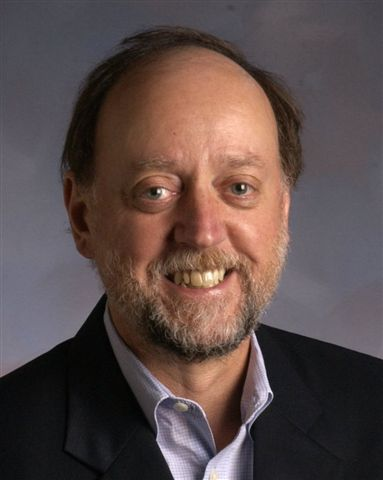
\includegraphics[width=3.8cm]{figures/JackDongarra.jpg}\\
        Prof. Jack Dongarra
      \end{center}
    \end{columns}
    \vfill
    \hrule
    \vskip0.2cm
    \footnotesize{Foto da \hyperlink{https://commons.wikimedia.org/w/index.php?curid=5234147}{Universidade do Tennessee, Knoxville}}
  \end{frame}
  
  \begin{frame}{FORTRAN/Fortran}
    \begin{columns}
      \column{0.45\textwidth}
      "I don’t know what the programming language of the year 2000 will look like, but I know it will be called FORTRAN.”
      \vfill
      \textemdash  Tony Hoare, ganhador do Turing Award de 1980, in 1982
      \column{0.45\textwidth}
      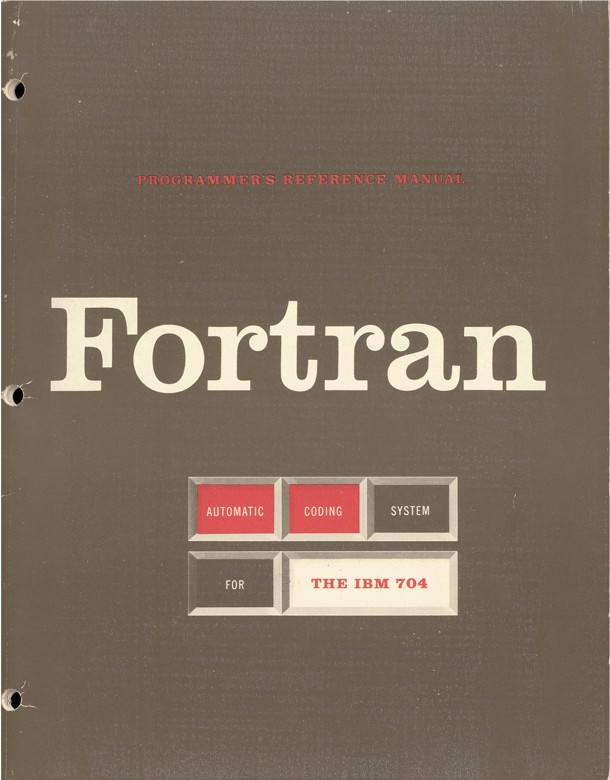
\includegraphics[width=5cm]{figures/Fortran_acs_cover.jpeg}
    \end{columns}
  \end{frame}
%  Wherever you see giant simulations of the type that run for days on the world’s most massive supercomputers, you are likely to see Fortran code. Some examples are atmospheric modeling and weather prediction carried out by the National Center for Atmospheric Research; classified nuclear weapons and laser fusion codes at Los Alamos and Lawrence Livermore National Labs; NASA models of global climate change; and an international consortium of Quantum Chromodynamics researchers, calculating the behavior of quarks, the constituents of protons and neutrons. These projects are just a few random examples from a large computational universe, but all use some version of Fortran as the main language.
  
  \begin{frame}[label=fortranslide]
    \frametitle{Como assim "Fortran Moderno?!"}
    \begin{figure}
      \centering
      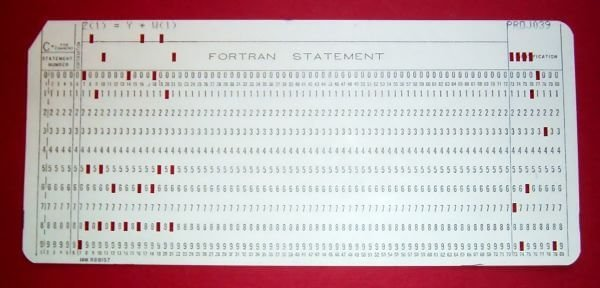
\includegraphics[width=0.5\textwidth]{figures/FortranCardPROJ039.jpg}
    \end{figure}
    \begin{itemize}
    \item FORTRAN 66/77, Fortran 90/95/2003/2008/2018 - \emph{backwards compatible}
    \item Código maduro, bibliotecas, interoperabilidade
    \item Arquiteturas variadas
    \end{itemize}
  \end{frame}
  
  \begin{frame}[label=features]
    \frametitle{Características}
    \begin{itemize}
    \item A estrutura de dados primária é o vetor/matriz
    \item Sintaxe de slicing nativa, masked arrays, vetorização$^*$
    \item É difícil escrever código lento! (\hyperlink{aliasing}{\emph{non-aliasing}})
    \item Fortran é \href{https://en.wikipedia.org/wiki/Concurrent_computing}{concurrent} desde 2008: \href{https://en.wikipedia.org/wiki/Coarray_Fortran}{coarrays} (com MPI)
    %This allows arrays to be split between processors for parallel processing, and it includes a natural syntax for interprocessor communication. With coarrays, parallel computation becomes part of the language specification rather than requiring a clumsy interface to an external library (although under the hood this is all actually implemented using MPI).
    \item Legibilidade: feito para computação científica
    \item Compiladores muito eficientes (alguns "roubando") \hyperlink{compilers}{\beamergotobutton{lista}}; 
    %For example, the Intel Fortran compiler can generate vector instructions and even message passing calls for optimized, distributed memory multiprocessing. The manufacturer, with intimate knowledge of the CPU, can ensure that the compiler produces machine code tuned to get the best possible performance from its architecture. Since supercomputers composed of their processing units will be compared with competitors using benchmarks written in Fortran, there is an economic and prestige-based motivation to invest in this level of compiler research and development.
    \end{itemize}
  \end{frame}
  
  \begin{frame}
    \frametitle{Futuro do Fortran}
    Ainda muito saudável em computação científica e HPC!

    \vfill
    Alguns projetos:
    \begin{itemize}
    \item CHARMM (Dinâmica molecular)
    \item Code$_{\ }$Saturne (Dinâmica de Fluidos Computacional)
    \item NEMO (Oceanografia)
    \item QUANTUMESPRESSO (Modelagem de Materiais)
    \item SPECFEM3D (Propagação de ondas sísmicas)
    \item WRF (Previsão do Tempo)
    \end{itemize}
    % Fonte: \href{https://www.quora.com/Is-FORTRAN-still-being-used-today-If-yes-what-do-people-use-it-for}{Lista de projetos em Fortran}
  \end{frame}
  
  \begin{frame}{E o Python? (Imagem de \cite{DataCamp})}
    \begin{center}
      \only<1>{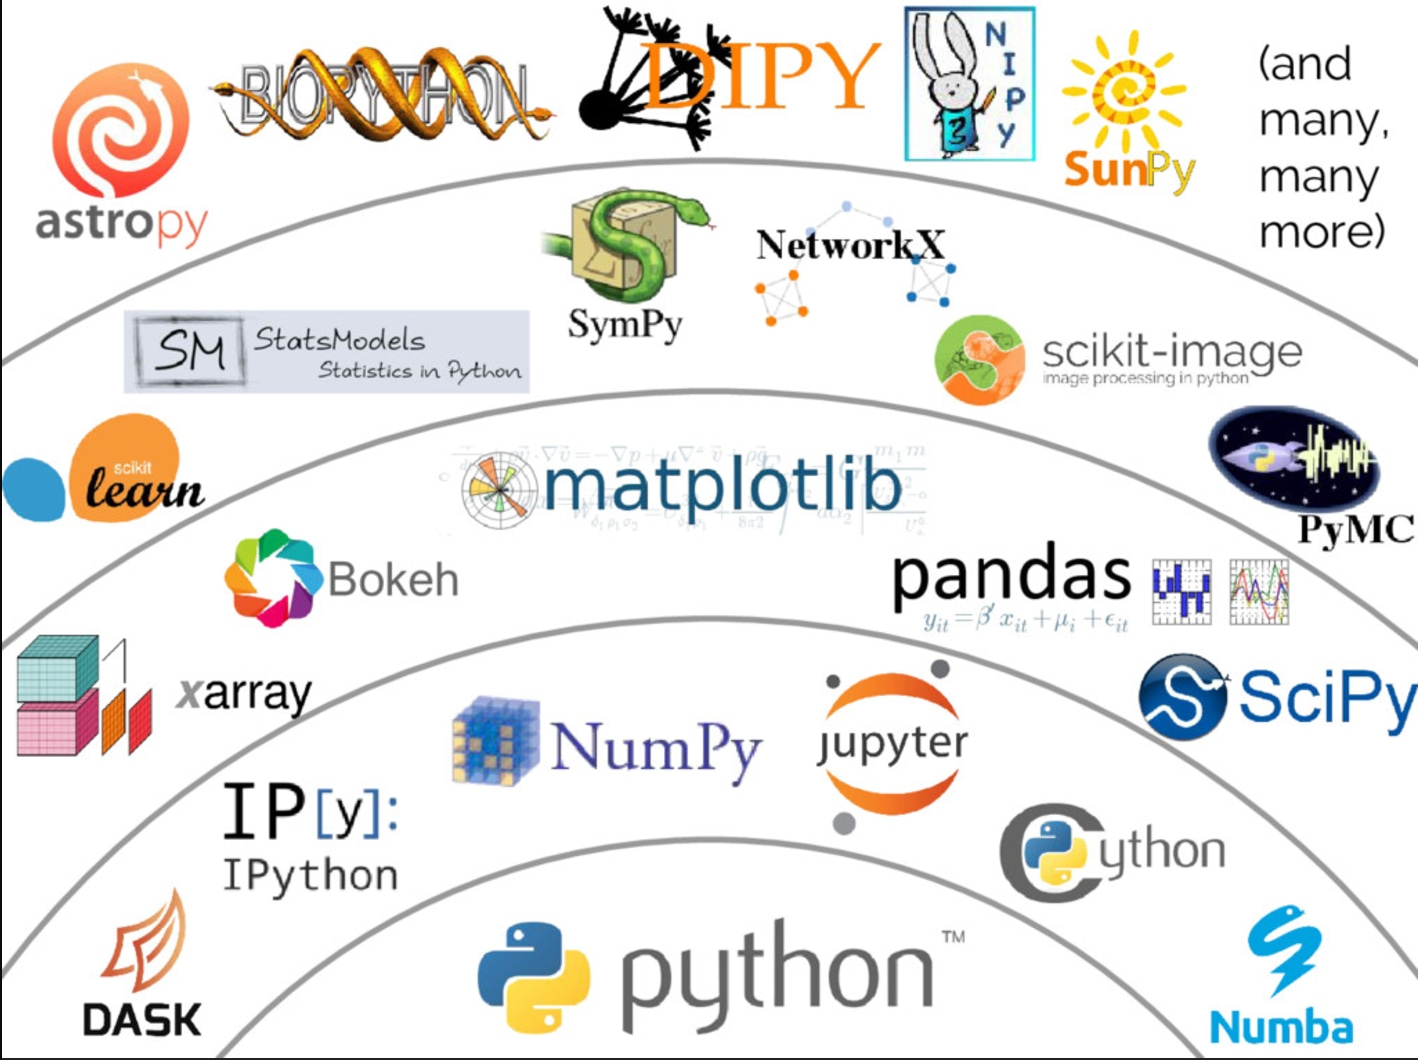
\includegraphics[width=8cm]{figures/scipy-eco_kqi2su.png}}
      \only<2>{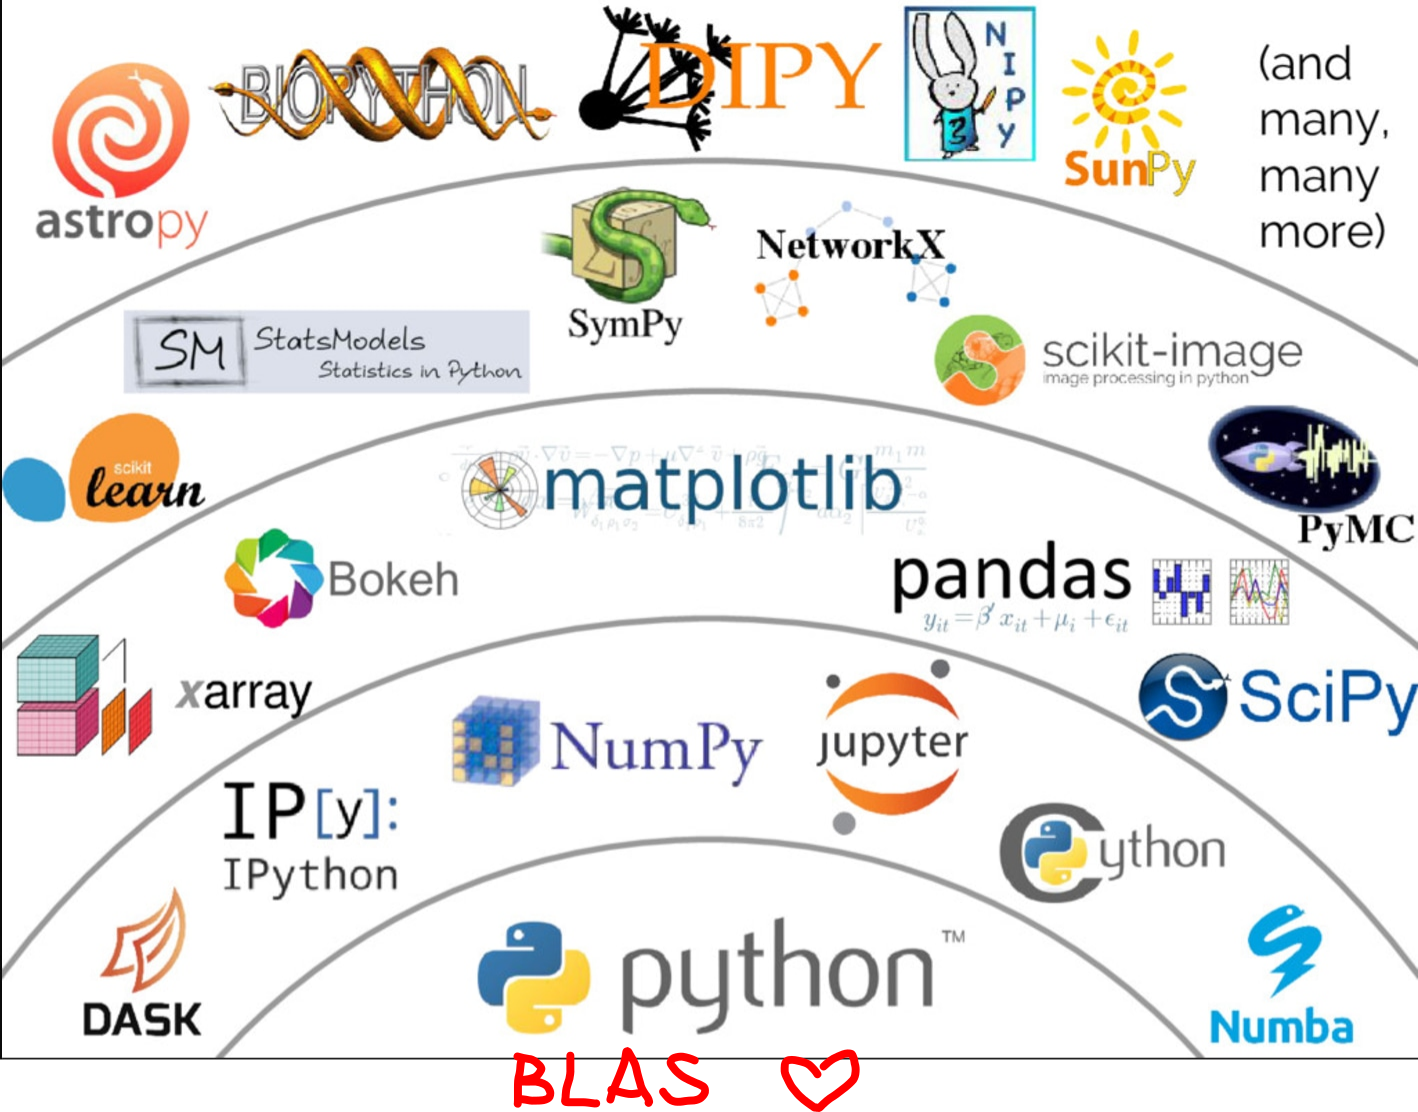
\includegraphics[width=8cm]{figures/scipy-eco_blas.png}}
    \end{center}
  \end{frame}
  
  \begin{frame}{Cython/Numba/Pypy}    
    \begin{itemize}
    \item<1-> É suficiente usar um JIT, ou acelerar o Python? \only<2->{Incompatíveis!}
    \item<3-> Perda de modularidade/interoperabilidade (código monolítico) 
      % higher level languages and problem-solving environments have resorted to a strategy of wrapping C++ and Fortran packages, and as described in a survey of differential equation solving suites
    \item<4-> Reescrever algoritmos especializados do zero?
    \item<5-> \only<5,7,8>{Numba}\only<6>{\alert{Numba}}
      \only<6>{%
        \begin{itemize}
        \item Fortran (SciPy) + Numba + Python ainda tem context switching 
          % From a function, Numba can generate native code for that function as well as the wrapper code needed to call it directly from Python. This compilation is done on-the-fly and in-memory.
        \item Não faz otimização interprocedural
        \item Determinar quando o código deve usar um JIT nem sempre é óbvio
          % It is worth noting that, as alluded to by Jörg, JIT is not necessarily invoked right away. Often, code will be interpreted until it is determined that it will be worth JITting. Since JITting can introduce delays, it may be faster to NOT JIT some code if it is rarely used and thus a fast response is more important than overall runtime.
        \end{itemize}
      }
    \item<5-> \only<5,6,8>{Cython}\only<7>{\alert{Cython}}
      \only<7>{%
        \begin{itemize}
        \item Linguagem compilada: compila Python em C.
        \item Grande parte da SciPy, pandas e scikit-learn estão escritas em Cython.
        \item Pode ser estaticamente tipada, e é aí que o desempenho melhora (loops em C)
        \item Pode desligar o GIL
        \end{itemize}
      }
    \item<5-> \only<5,6,7>{Pypy}\only<8>{\alert{Pypy}}
      \only<8>{%
        \begin{itemize}
        \item JIT (RPython)
        \item GIL: existem workarounds, mas não tão eficientes
        \item Grande parte da SciPy, pandas e scikit-learn estão escritas em C(ython).
        \end{itemize}
      }
  \end{itemize}    
  \end{frame}

  \begin{frame}
    \frametitle{E o C?}
    \begin{center}
      \begin{block}{}
        \small{``C is pretty much a model of the computer, where you can glue on as much linear algebra as you want, provided you are prepared to pretend that it resembles the computer.

        Fortran is pretty much a model of linear algebra, where you can glue on as many computer details as you want, provided you are prepared to pretend that they resemble linear algebra.

        % In the end, they both turn into machine code, and the resultant binary goodness is directly proportional to how far you have been able to see through what your compiler is up to.
        (...)
        
        \textbf{Whether you prefer to pretend that the computer is made of linear algebra or that the linear algebra is made of computer, depends mostly on where you are coming from to begin with.}''}
      \end{block}
    \end{center}
    \begin{flushright}
      \vskip-0.7cm
      \hskip3cm \textemdash \ \footnotesize{Resposta em \cite{quora}}
    \end{flushright}
  \end{frame}

  \begin{frame}
    \frametitle{E o C++?}
    \begin{itemize}
    \item Blitz++: expression templates, template metaprogramming
    \item Já é possível escolher non-aliasing
    \item Sem garbage collection (assim como o Fortran, mas naturalmente usa-se mais ponteiros do que no Fortran)
    \item Reprodutibilidade?
    \end{itemize}
  \end{frame}
  
  \begin{frame}{HPC}
    Em uma \href{https://software.intel.com/en-us/blogs/2015/03/27/doctor-fortran-in-the-future-of-fortran}{pesquisa*} de usuários de Fortran na 2014 Supercomputing Convention, 100\% dos entrevistados disse que acreditavam que ainda estariam usando Fortran em 5 anos.
    \begin{itemize}
    \item C++ e Fortran moderno, com OpenMPI
    \item CUDA
    \item Clay Christiansen, em ``The Innovators Dillema'' diz que tecnologias disruptivas aparecem quando surge um novo mercado/grupo de usuários
    \item Loop fission/fusion, multithreading, coarrays não são \emph{nice to have}; são \textbf{essenciais}!
    \item Exemplos: \url{http://www.archer.ac.uk/status/codes/}
      % LU factorization benchmark https://www.ibm.com/developerworks/community/blogs/jfp/entry/A_Comparison_Of_C_Julia_Python_Numba_Cython_Scipy_and_BLAS_on_LU_Factorization?lang=en      
    \end{itemize}
  \end{frame}
  
  \begin{frame}
    \frametitle{Julia: a solução para o problema das duas linguagens?}
    \centering
    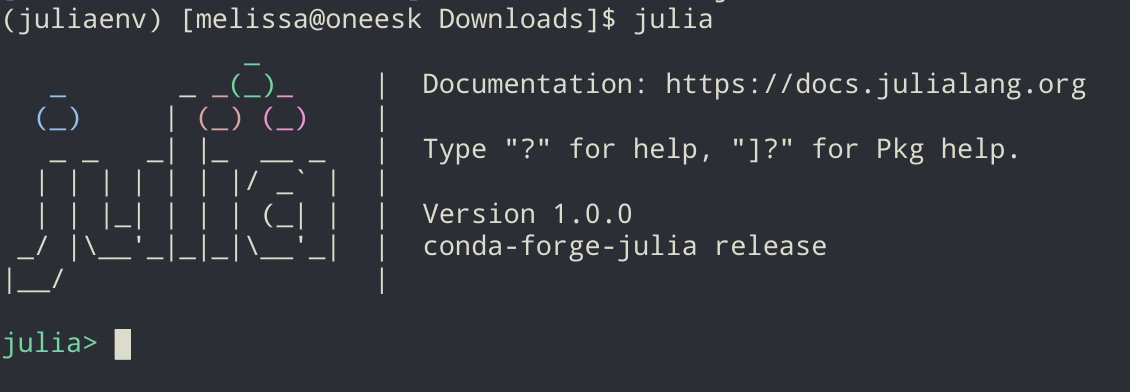
\includegraphics[width=8cm]{figures/juliaconsole.png}
    \begin{itemize}
    \item<2-> Não é um Python mais rápido, e sim um C++ mais produtivo
    \item<3-> Mais próximo de um AOT do que de um JIT
    \item<4-> ``We believe that the traditional HPC and “Big Data” worlds are converging, and we’re aiming Julia right at that convergence point.'' (Stefan Karpinski, Viral Shah, Jeff Bezanson and Alan Edelman)
    \end{itemize}
  \end{frame}
  
  \begin{frame}[fragile]
    \frametitle{Julia II: Revenge of the Loops}
    \begin{itemize}
    \item<1-> Ideia principal: Multiple Dispatch + Estabilidade de Tipos => Velocidade + Legibilidade
      % Multiple dispatch is the language feature that really sets Julia ahead of the pack for numerical computing. Mathematical code tends to separate into high-level generic algorithms that could be applied to lots of different implementations of numeric types and structures on the one hand and very specialized custom implementation of those numeric types and operations on the other. Multiple dispatch is what lets you join these together smoothly—it lets you separate the usage of an abstraction from implementations of it, cleanly, in a way that we’ve never encountered in other systems.
    \item<2-> LLVM permite competitividade em máquinas de todos os tipos
      % “Big Iron” machines (think IBM, Cray) used in high-performance computing (HPC) circles often have only C or Fortran compilers. But with new projects like LLVM, it’s increasingly possible to get good compiler support for many different languages on new hardware just by adding a new backend for LLVM—which is significantly easier than writing a C compiler from scratch. Recently, for example, someone got Julia running on ARM and we did nothing special to make that possible.
      %%%% 
      % Stefan Karpinski, Viral Shah, Jeff Bezanson, and Alan Edelman—were kind enough to respond to some questions by e-mail. On the subject of concurrency, they say:
      % Julia makes it easy to connect to a bunch of machines—collocated or not, physical or virtual—and start doing distributed computing without any hassle. You can add and remove machines in the middle of jobs, and Julia knows how to serialize and deserialize your data without you having to tell it. References to data that lives on another machine are a first-class citizen in Julia like functions are first-class in functional languages. This is not the traditional HPC model for parallel computing but it isn’t Hadoop either. It’s somewhere in between.
    \item<3-> Interoperabilidade com Fortran, C, Python
    \item<4-> Metaprogramming, code introspection
    \item<5-> Desempenho previsível: IR legível \verb+@code_llvm+, \verb+@code_native+
    \item<6-> Multiparadigmas
      % https://stackoverflow.com/questions/20613817/julia-julia-lang-performance-compared-to-fortran-and-python
      % \item precompiled modules (.ji files).
      % \item This is another interesting feature of Julia: it lets you by default have the safety of a scripting language, but turn off these features when necessary (/after testing and debugging) to get full performance. (\verb+@inbounds+)
      % \item But lastly, using this strategy Julia actually can produce static binaries like compiled C or Fortran code, so I think this fact will come in handy for making Julia into a package development language. Basically, you can write packages in Julia, and someday it will be easy to generate a runtime-free binary (like C/Fortran) others can link to.
    \end{itemize}
  \end{frame}
  
  \begin{frame}{Julia III: Computação Científica Edition}
    \begin{itemize}
    \item O esquema de compilação facilita o desenvolvimento de software científico
    %\item ``Sure, if someone wrote a very large software in Fortran which is perfectly optimal, Julia probably can’t optimize that as well as Fortran because it can alias pointers among other things which can disable some compiler optimizations. However, without any pain, Julia will get you <2x from Fortran. Using some macros to create little local environments that are aliasing free and things like that, Julia can probably get stupidly close to Fortran (like <1.2x) with minimum work (probably 10x-100x less code...).''
     \item \emph{A maior parte das pessoas não consegue escrever “Fortran ótimo”}. Cientistas não são engenheiros de software.
     %\item Most of these benefits will be seen by package developers. "Users" will probably not see as much of a difference in their own codes because the majority of their performance will be determined by the packages they use.
     \item Para scripts pequenos o benefício pode não ser óbvio
     \item Para desenvolvedores de pacotes de computação científica, pode ser revolucionário!
     \end{itemize}
   \end{frame}

   \begin{frame}[fragile]
     \frametitle{Julia Paralelo, HPC, e para Ciência de Dados: Pacotes}
     % \item state of the art julia packages https://discourse.julialang.org/t/what-package-s-are-state-of-the-art-or-attract-you-to-julia-and-make-you-stay-there-not-easily-replicateable-in-e-g-python-r-matlab/11294/4
     \begin{itemize}
     \item Paralelização simples: \verb+@threads+ paraleliza loops; \verb+@parallel+ adiciona a possibilidade de utilizar multiprocessamento
     \item \verb+CUDAnative.jl+, \verb+GPUArrays.jl+ 
     %\item \url{https://nextjournal.com/sdanisch/julia-gpu-programming}
     %\item \url{https://devblogs.nvidia.com/gpu-computing-julia-programming-language/}
     \item \verb+Flux.jl+, \verb+Knet.jl+ para ML
     \item \verb+DifferentialEquations.jl+
     \item \verb+IterativeSolvers.jl+ (Matrix-free; \verb+A_mul_B+)
     \item \verb+Convex.jl+, JuMP, JuliaSmoothOptimizers
     \item \url{https://juliaobserver.com/}
    \end{itemize}
  \end{frame}

  \section{Challenges}
  \begin{frame}
    \frametitle{Desafios Técnicos}
    \begin{itemize}
    \item<2-> Obter o desempenho dos benchmarks nem sempre é fácil!
    \item<3-> ``Better software, better research'': será que a velocidade é sempre o mais importante?
    \item<4-> Poderio computacional não é tudo: algoritmos podem ser mais importantes que a implementação
    \item<5-> Clojure? Haskell? Linguagens Funcionais? Ainda não tiveram sucesso na Computação Científica (cópias; dados imutáveis; funções puras) 
    %Immutable data makes it easier to reason about code and to write correct concurrent programs. However, these very advantages lead to problems when trying to do computational physics in the large. Fast, large-scale numerical code depends on destructive updating of large arrays. This goes against the grain of the functional approach. Haskell and Clojure can be coerced to hack on memory locations, but at the cost of sacrificing many of their natural idioms and even violating their philosophies. Hickey, the author of Clojure, emphasizes the distinction between place and value, suggesting that computation should be thought of as the transformation of the latter. But fast numerics would seem to require dealing with place in the sense of locations in arrays.
    %The Julia team offered these salient remarks in response to a question about the possible roles of Haskell and Clojure: ``When you have, for example, a huge array—one that barely fits in memory—you can’t really afford to make any copies of it or represent it as anything besides a big contiguous chunk of mutable memory. For really hard computational problems, it is often the case that the only known tractable algorithms make extensive, essential use of mutable state. In a sense, Clojure and Haskell are tackling some of the hardest problems in computer science while Julia is aimed at the hardest problems in computational science. Someday, we may know how to deal with both at the same time, but for now, I think we have to choose our battles.''
    \end{itemize}
  \end{frame}

  \begin{frame}{Desafios menos técnicos}
    \begin{itemize}
    \item<1-> Padrões e linguagens novas nem sempre são adotados rapidamente
    \item<2-> \emph{Research Software Engineers}%: "An article about computational result is advertising, not scholarship. The actual scholarship is the full software environment, code and data, that produced the result." -- Buckheit and Donoho, 1995
    \item<3-> Desempenho numérico em grande escala é um problema difícil e particular %, e somente as linguagens especificamente projetadas para estes problemas tem sido capazes de lidar com essa problemática.
    %\cite{arstechnica}
    \item<4-> É difícil convencer pessoas a trabalharem em projetos open source porque o desenvolvimento de software não é visto como um produto de pesquisa válido para acadêmicos. ``Toda grande biblioteca matemática open source é construida sobre as cinzas da carreira acadêmica de alguém''.
    %\item What we needed was a new way to connect software development to the mathematics so that we can get the newest/fastest methods into the hands of those who need them while keeping in line with academic incentives (publications and grants).
    \end{itemize}
  \end{frame}
  
  \section{References}
  \begin{frame}[label=bibliography, allowframebreaks]{Bibliografia}
    \scriptsize{%
    \begin{thebibliography}{99}
    \bibitem{GolubOrtega}
      Gene H. Golub and James Ortega. \emph{Scientific Computing and Differential Equations \textemdash\ An Introduction to Numerical Methods}. Academic Press, 1992.
    \bibitem{TUKweb} \emph{What is Scientific Computing?} \hyperlink{https://www.scicomp.uni-kl.de/about/scientific-computing/}{Technische Universität Kaiserslautern}
      
    \bibitem{DataCamp} \emph{Python Scientific Computing} \hyperlink{https://www.datacamp.com/community/blog/python-scientific-computing-case}{DataCamp}
       
    \bibitem{arstechnica} \emph{Scientific Computing's Future: Can any coding language top a 1950's behemoth?} \hyperlink{https://arstechnica.com/science/2014/05/scientific-computings-future-can-any-coding-language-top-a-1950s-behemoth/}{Ars Technica}
    
    \bibitem{numbajulia} \emph{Why Numba and Cython are not substitutes for Julia} \hyperlink{http://www.stochasticlifestyle.com/why-numba-and-cython-are-not-substitutes-for-julia}{Stochastic Lifestyle Blog}
    
    \bibitem{comparison} \hyperlink{https://www.hindawi.com/journals/sp/2014/870146/abs/}{\emph{Formula Translation in Blitz++, NumPy and Modern Fortran: A Case Study of the Language Choice Tradeoffs}}
    %\bibitem{introtojulia} \url{http://ucidatascienceinitiative.github.io/IntroToJulia/}
    %\bibitem{thinkjulia} \url{https://benlauwens.github.io/ThinkJulia.jl/latest/book.html}
    \bibitem{quora} \hyperlink{https://www.quora.com/For-scientific-computing-what-are-the-advantages-and-disadvantages-of-using-C-as-compared-to-using-FORTRAN-90}{\emph{For scientific computing, what are the advantages and disadvantages of using C as compared to using FORTRAN 90?}}
    \end{thebibliography}
    }
  \end{frame}
  
  \section{Appendix}
  
  \begin{frame}[label=compilers]
    \frametitle{Fortran Compilers}
    \begin{itemize}
    \item GFortran
    \item Flang: LLVM
    \item Intel ifort: \href{https://en.wikipedia.org/wiki/SIMD}{SIMD} vetorização e threading, OpenMP
    \item Lahey/Fujitsu
    \item NAG
    \item IBM XL Fortran: SIMD, OpenMP, Arquitetura Power9
    \item Arm Fortran Compiler
    \end{itemize}
    \hyperlink{features}{\beamergotobutton{back}}
    \addtocounter{framenumber}{-1}
  \end{frame}
  
  \begin{frame}[label=aliasing]
    \frametitle{Aliasing}
    \footnotesize{``Fortran, by forbidding aliasing, holds a significant advantage over C++. Aliasing means that if a Fortran function gets two arrays, slices, or values, modifying one of them is assumed not to affect the other. If the programmer accidentally passed two parameters that alias, there is no guarantee that the result will be correct. Fortran basically passes the responsibility to the programmer, while C++ tries to be safer. The impact on performance can be devastating for C++. In Fortran, because parameters are not supposed to alias, the compiler can keep a value from parameter A in a register even when it writes data to parameter B. In C++ this does not work this way, since the compiler can’t always be sure if writing to B is guaranteed to not touch A. So C++ has to reload the value in the register of A, from memory every time. Here is where C is better than C++. In C it is possible to mark a parameter with restrict to signify that it can’t alias, and get performance similar to Fortran for a single function. This keyword is not available in C++.''}
    \vfill
    \textemdash\ from \href{https://www.quora.com/Is-there-something-fundamental-to-the-Fortran-language-itself-not-massive-legacy-code-bases-or-time-proven-optimizing-compilers-that-causes-it-to-still-be-preferable-to-speed-critical-numerical-computations-HPC}{Is there something fundamental to the Fortran language itself (not massive legacy code bases or time-proven optimizing compilers) that causes it to still be preferable to speed-critical numerical computations/HPC rather than, say, C/C++?}

    %See https://stackoverflow.com/questions/146159/is-fortran-easier-to-optimize-than-c-for-heavy-calculations
    \hyperlink{features}{\beamergotobutton{back}}
    \addtocounter{framenumber}{-1}
  \end{frame}
  
\begin{frame}{LLVM}
  \begin{itemize}
  \item LLVM is an umbrella project of low-level compiler toolchain components. It is written in C++  
  \item LLVM can be used as a compiler framework, where you provide the "front end" (parser and lexer) and the "back end" (code that converts LLVM's representation to actual machine code).
  \item LLVM can also act as a JIT compiler - it has support for x86/x86$_{\ }$64 and PPC/PPC64 assembly generation with fast code optimizations aimed for compilation speed.
  \item LLVM is famous for its Intermediate Representation (IR) and IR Optimizer.
  \item Some languages use C as IR: Python
  \item LLVM's IR is a low-level programming language, similar to assembly. It is a strongly typed RISC-like instruction set.
  \item LLVM's IR Optimizer allows various input languages to be transformed to machine code to various architectures
  \item The IR Optimizer eliminated redundancy by looking at the structure of the IR
  \item LLVM is great as a compiler backend for statically-typed compiled languages, but it has been known not to work equally well in the context of dynamic languages; some projects are moving away from it      
  \end{itemize}
  \addtocounter{framenumber}{-1}
\end{frame}
 
\begin{frame}{SIMD Vectorization}
  \begin{itemize}
  \item Single instruction, multiple data (SIMD) is a class of parallel computers in Flynn's taxonomy
  \item From \href{https://en.wikipedia.org/wiki/SIMD}{Wikipedia}: \emph{"It describes computers with multiple processing elements that perform the same operation on multiple data points simultaneously. Such machines exploit data level parallelism, but not concurrency: there are simultaneous (parallel) computations, but only a single process (instruction) at a given moment. SIMD is particularly applicable to common tasks such as adjusting the contrast in a digital image or adjusting the volume of digital audio. Most modern CPU designs include SIMD instructions to improve the performance of multimedia use. SIMD is not to be confused with SIMT, which utilizes threads."} 
  \end{itemize}
  \addtocounter{framenumber}{-1}
\end{frame}

\end{darkframes}

\end{document}

%https://www.scivision.dev/speed-of-matlab-vs-python-numpy-numba/